\chapter{Machine Learning Background}\label{chap:ml}

\begin{figure}[h]
    \centering
    \includegraphics[width=0.8\linewidth]{Chapters/Theoretical_Background/images/eggholder.pdf}
    \caption{A gradient descent trajectory failing to optimise to global minima on the Eggholder function.}
    \label{fig:eggholder}
\end{figure}

The name machine learning, combined with its current overuse, can sometimes be misleading. Machine learning methods need no modern machines as we know them today. Given a pen, paper, and enough time, anyone can do machine learning. More precisely, what these methods do need is a computational machine - be it a human or a modern computer. Of course, the computer here would have an advantage in terms of automation and floating-point operations per second, and that is why we use them.

We will often refer to machine learning as statistical learning, as this name is more informative and helps to reduce some mysticism around the field.

\blindmathtrue
\section{Statistical Learning}

Statistical learning involves utilising statistics to extract knowledge from data. We therefore must clarify the meaning of data and learning in this context. First, there are various types of learning, typically categorised into supervised, unsupervised, and reinforcement learning. In supervised learning, the aim is to create a model that takes labelled examples as input and predicts outputs. The goal of unsupervised learning is to identify patterns or structures within the data, without explicit labels in the inputs. Lastly, reinforcement learning is distinct in that an agent makes decisions and interacts with an environment to obtain rewards based on its actions.

Consider a function $f :  X \to Y$, where $X$ is a set of possible inputs with $Y$ the set of all possible outputs. Here, data refers to subsets or sample vectors $x_i$ and $y_i$ from the respective sets, which makes $\{x_i, y_i\} \in X \times Y$. Learning, then, is the process of creating a model $\hat{f}(x_i)$ that model $f$ up to some error $\epsilon$,
\begin{align*}
    \hat{f}(x_i) = y_i + \epsilon_i.
\end{align*}

The error, or noise term, is a deviation of the model prediction from the actual output, and can occur from inherent fluctuations of the dataset or limitations of the model itself. In the case of an idealised model $\hat{f}$, we assume that $\epsilon$ follows a normal distribution $\mathcal{N}$, which is motivated by the law of large numbers.

Training a model involves searching for a model which minimises this error as much as possible. We are, however, free to choose how this error is measured, and, as we will discuss, that will greatly influence the minimisation search. For now, let us simply state that such a function, which represents a distance between the model's prediction and ground truth, should map to a real number. We will call it a loss function $\mathcal{L : \mathcal{H}} \to \mathbb{R}$, with $\mathcal{H}$ a set of all possible functions from input to output space\footnote{Note that this is not just any function, as the type of model adds constraints: it could be linear model, neural network, and so on.}. For now, we simply write
\begin{align}
    \mathcal{L}(f, \mathcal{D}) \propto \sum_{(x_i, y_i)\in \mathcal{D}}d(f(x_i), y_i),
    \label{eq:loss_as_average}
\end{align}
where $\mathcal{D} \subset X\times Y$, and $d$ a measure of the distance of the individual predictions to the truth. For now, it suffices to state that it will be a convex function such as the mean squared error.

\subsection{Learning as \MakeLowercase{a}n Optimisation Problem}\label{subsec:Learning as opt}

To quote Bennett \cite{bennett2006interplay}, ``Optimization problems lie at the heart of most machine learning approaches''. On that note, the objective of our learning is to find a function that, given a data set $\mathcal{D} = \{(x_i, y_i)\}$ from a hypotesis space $\mathcal{H}$, minimises $\mathcal{L}$. In mathematical terms, the problem becomes
\begin{align}
    \min_{f \in \mathcal{H}}\mathcal{L}(f, \mathcal{D}).
    \label{eq:min_prob}
\end{align}

However, this is only part of the problem. In statistical learning, we want models capable of generalising to unseen data. We want models to learn general features of datasets, rather than hyper-specialising on a specific one. This discussion is central to supervised learning and is deeply related to the concept of bias-variance trade-off, better discussed in \cite{hastie2009elements}. This specialisation process usually comes with an increase in complexity of the model, which leads to a higher variance, albeit smaller bias in the prediction values. To better estimate that, one usually breaks the data set into a training and testing set. Here we deliberately avoid that discussion as this technique is not used in our methods.

\section{Gradient-based Optimisation}\label{sec:Gradient-based optimisation}
There are several ways to approach optimisation problems, such as the one described in Section \ref{subsec:Learning as opt}. The technique of choice depends on the nature of the problem at hand, but perhaps the most famous is gradient-based optimisation. For a large class of problems, many functions we want to minimise - or maximise - are based on physically or statistically reasonable functions. For that reason, they are frequently well behaved in the differential calculus sense. If a specific loss function is sufficiently smooth\footnote{has well deffined derivatives up to some order $k$ over some domain $\mathcal{D}$. }, and has an extrema (minimum or maximum) at some point in the domain, we know $\nabla\mathcal{L} = 0$. 

Note how the domain of $\mathcal{L}$ is a very general vector space of functions. To make the differentiation process more intuitive, we parameterise a model $f_{\mvec{\theta}}: X \to Y$. This means that after fixing a functional form, we can explore the hypothesis space by changing the parameters $\mvec{\theta}$, and so the optimisation quest becomes
\begin{equation}
\mvec{\hat{\theta}} = \text{arg}\min_{\mvec{\theta}} \mathcal{L} (f_{\mvec{\theta}}, \mathcal{D}).
\label{eq:optimisation}
\end{equation}

\subsubsection{Steepest Descent}\label{sub:steepest}
The idea behind steepest descent (SD) is to iteratively update $\mvec{\theta}$ in a direction that minimises $\mathcal{L}$ and to do so using the gradient of the loss with respect to the parameters. The motivation is simple: this gradient should be related to the direction in which $\mathcal{L}$ decreases the most for the smallest displacement $\mvec{\delta}_{\theta} = \mvec{\theta}_{t+1} - \mvec{\theta}_{t}$. The word ``related'' carries a significant conceptual weight here, especially because we have not defined how to measure such displacement. For now, we shall use the Euclidean norm, in which case we write
\begin{equation*}
d\left(\mvec{\theta}_{t+1}\,,\,\mvec{\theta}_{t}\right)\,=\,\norm{ \mvec{\delta}_{\theta}}_2.
\label{eq:dist}
\end{equation*}

Our wordy motivation for steepest descent can then be written mathematically if we first take a first order approximation of $\mathcal{L}$ around $\mvec{\theta}_{t}$:
\begin{equation}
    \mathcal{L}(\mvec{\theta}) \approx \mathcal{L}(\mvec{\theta}_{t}) +  \mvec{\delta}_{\theta}^\top \nabla \mathcal{L}(\mvec{\theta}_{t}).
    \label{eq:taylor}
\end{equation}

Performing an iterative minimisation with the smallest possible step can be posed as a constraint minimisation problem. If we set the distance to an arbitrary but fixed scalar, $d\left(\mvec{\theta}_{t+1}\,,\,\mvec{\theta}_{t}\right)\,= \epsilon$, the quest for the optimal parameter can be written
\begin{align}
    \mvec{\theta}_{t+1}\,=\arg \min_{\mvec{\theta}}\left[\mathcal{L}(\mvec{\theta}_{t}) +  \mvec{\delta}_{\theta}^\top\nabla \mathcal{L}(\mvec{\theta}_{t})\,+\, \epsilon \right].
    \label{eq:steepst_argmin}
\end{align}

We have constrained the minimization of $\mathcal{L}$  to a function $d$, which can be solved via Lagrange multipliers (see Appendix \ref{appendix:steepest}), yielding
\begin{equation}
\mvec{\theta}_{t+1} = \mvec{\theta}_t - \alpha \nabla \mathcal{L}(\mvec{\theta}_t)    .
\label{eq:gradient_rule}
\end{equation}

The parameter $\alpha$, called the learning rate, is a scaling factor from the Euclidian distance, together with the displacement constraint $\epsilon$. In real-life applications, we often choose such a parameter experimentally. Using too big of a learning rate will mean that the constraint has not been satisfied, and steps are taken outside of the trust region which guarantees the linear approximation of the method.

Steepest descent has some pitfalls. First, all directions in parameter space are treated equally, in terms of scale, by the fixed learning rate. Depending on the parametrisation of our cost function, this might be a terrible assumption. Second, the learning rate is fixed; then, a large learning rate might make it impossible to reach convergence. Note that employing an extremely small learning rate is not practical either, as it would require more iterations to reach convergence and inevitably more computational time. Hereafter we will discuss some of the techniques to try and address these points. 

\subsubsection{Newton's Method}

The most immediate way to address the problem of equal treatment of the parameter scale is to use a higher-order Taylor expansion in \eqref{eq:taylor}. This is the essence of Newton's method. In this case, the update rule guided by the minimisation is expressed as 
\begin{equation}
\mvec{\theta}_{t+1} = \arg \min_{\mvec{\theta}} \left[\mathcal{L}(\mvec{\theta}_t) +  \mvec{\delta}_{\theta}^\top \nabla \mathcal{L}(\mvec{\theta}_t) + \frac{1}{2}  \mvec{\delta}_{\theta}^\top \text{H}(\mvec{\theta}_t)  \mvec{\delta}_{\theta} + \epsilon \right],
\label{eq:newtons_minimisation}
\end{equation}
for which the update rule becomes
\begin{align}
\mvec{\theta}_{t+1} &= \mvec{\theta}_t - \alpha \text{H}^{-1}(\mvec{\theta}_t)\nabla \mathcal{L}(\mvec{\theta}_t)\\  
\text{H}(\mvec{\theta}_t)&=\nabla^2 \mathcal{L}(\mvec{\theta}_t)
\label{eq:newtons_method}
\end{align}
where $\text{H}$ is the so-called Hessian matrix.

Newton's method improves the step towards the direction of the negative gradient of the loss function by adding information of the curvature of the objective function $\mathcal{L}$ via the Hessian matrix. While several of the theoretical arguments behind both SD and Newton's method are tailored to convergence in a convex landscape, they can be used in non-convex problems with some caution and techniques.

Convex functions are characterised by the property that the line segment connecting any two points on the function's graph always remains above the graph itself. A classical example being a parabola, optimisation on those functions is straightforward, as any local minima are also global minima. In contrast, non-convex functions do not have this guarantee, due to the potential presence of several local-minima or saddle points. In the latter class of functions, having bad initialisation points can in the worst scenario lead to divergence in the algorithm or lead to convergence to local minima. 

At this point, one might ask why not always use Newton's method. As for most computational problems, the answer is both storage and computational efficiency. The Hessian matrix is quadratic in number of parameters and has to be updated and stored for every iteration of the training process. Calculating the elements of the matrix is also expensive, since it involves the double derivatives of the objective function, and finally, inverting a matrix also has approximately cubic complexity. 

\subsubsection{Momentum Gradient Descent} 

The steepest descent method of Subsection \ref{sub:steepest} with update rule given by \eqref{eq:gradient_rule}, can be rewritten as
\begin{align*}
    \mvec{\delta}_t &= \alpha \nabla_{\mvec{\theta}} \mathcal{L}, \\
    \mvec{\theta}_{t+1} &= \mvec{\theta}_{t} - \mvec{\delta}_t .
\end{align*}

A simple improvement in this method is the addition of a moment term $\gamma \in (0,1)$. This parameter controls the maintenance of some information, or memory, about the convergence behaviour of the parameter update in previous epochs. The analogy arises as the moment of a particle increases, while its potential energy on a downward trajectory is minimised. The intuitive argument for this analogy is that, by having moment, such a particle traversing a landscape is able to overcome potential local minima or move ever so fast when in regions with a steady downhill trajectory. Following this reasoning, the algorithm follows
\begin{align*}
    \mvec{\delta}_t &= \gamma \mvec{\delta}_{t-1}  + \alpha\nabla_{\mvec{\theta}} \mathcal{L}, \\
    \mvec{\theta}_{t+1} &= \mvec{\theta}_{t} - \mvec{\delta}_t.
\end{align*}

This is an exponentially weighted average of displacements along the epochs, with the moment term $\gamma$ controlling how much to remember from the previous iterations. This constant is therefore a number between 0 and 1, to be fine-tuned experimentally. Note that this memory term invariably contains some information about the curvature of the landscape, while still being part of a first-order method.

\subsubsection{Root Mean Squared propagation (RMSprop)}

We have mentioned that a constant learning rate can affect the convergence of the training. We now present two examples among the class of adaptative learning rate methods that attempt to address this problem.

To avoid the computational cost of taking the second derivative of the loss function, RMSProp \cite{graves2013generating} aims at correlating this information with the moving average on the squared gradient of each parameter, represented here as $\mvec{s}_t$, and modulated by a decay rate $\beta$. This method assigns individual effective learning rates for each parameter and also modulates them by a decay rate. This makes the algorithm move fast in the beginning (large learning rate) when we are probably distant from the minima, and then proceed with caution as we hope to approach convergence:
\begin{align*}
    \mvec{s}_t &= \beta \mvec{s}_{t-1}  + (1- \beta)(\nabla_{\mvec{\theta}} \mathcal{L}\odot \nabla_{\mvec{\theta}} \mathcal{L}), \\
    \mvec{\theta}_{t+1} &= \mvec{\theta}_{t} -  \frac{\alpha}{\sqrt{\mvec{s}_t + \epsilon}} \odot \nabla_{\mvec{\theta}}\mathcal{L},
\end{align*}
where $\epsilon$ serves as a stability factor to avoid division by 0, and is usually a number around $10^{-9}$.

\subsubsection{Adaptative Moment Estimation (Adam)} 

Another widely used method that takes into account the second moment of that gradient is Adam or Adaptive Moment Estimation \cite{kingma2014adam}. In contrast to RMSProp, Adam considers both the first order ($\mvec{m}_t$) and the second order moment ($\mvec{s}_t$) of the gradient of each parameter, being a combination of momentum GD and RMSProp. Adam further includes bias corrections to these moments, denoted respectively $\mvec{\hat{m}}_t$ and $\mvec{\hat{s}}_t$. We will not derive the expression of these corrections, but the original authors of the paper argue for their motivation: since the first- and second-moment terms are exponentially weighted averages, their initialisation value of zero inevitably introduces a bias into their accumulation value. 

Adam has been shown to be an extremely robust optimisation algorithm, which means that it performs well in a wide class of different problems \cite{reyad2023modified, zhang2022adam}. For our use and purposes, we simply state the update rules below,
\begin{align*}
    \mvec{m}_t &= \beta_1 \mvec{s}_{t-1}  + (1- 
    \beta_1)\nabla_{\mvec{\theta}} \mathcal{L}, \\
    \mvec{\hat{m}}_t &=  \frac{\mvec{m}_t}{1- \beta_2^t}, \\
    \mvec{s}_t &= \beta_2 \mvec{s}_{t-1}  + (1- \beta_2)(\nabla_{\mvec{\theta}} \mathcal{L}\odot \nabla_{\mvec{\theta}} \mathcal{L}), \\
    \mvec{\hat{s}}_t &= \frac{\mvec{s}_t}{1- \beta_2^t}, \\
    \mvec{\theta}_{t+1} &= \mvec{\theta}_{t} - \frac{\alpha}{\sqrt{\mvec{\hat{s}}_t} + \epsilon} \odot \mvec{\hat{m}}_t.
\end{align*}

Note that the first and second moments are modulated by different constants $\beta_1$, $\beta_2$, while $\epsilon$ has the same role as in RMSProp.

\subsection{Stochastic Gradient Descent}\label{section:sgd} 

Up to this point, the discussion about statistical learning had as a cornerstone the minimisation of the loss of \eqref{eq:min_prob}, evaluated throughout the dataset $\mathcal{D}$. In reality, most deep learning methods are conducted with an evaluation of the loss and respective gradients on subsets of the dataset. This technique is adopted not only for efficiency benefits but also for its impact on convergence. To illustrate it, we recall the simple update rule for the steepest descent, in \eqref{eq:gradient_rule}. For the calculation of the gradient, the proportionality of \eqref{eq:loss_as_average} can be turned into equality by choosing a mean squared error approach. Recalling also that we are solving a parametrised problem, we write
\begin{align}
    \nabla_{\mvec{\theta}} \mathcal{L}(\mvec{\theta}) &= \frac{1}{\left| D\right|}\sum_{(x_i, y_i) \in \mathcal{D}} \nabla_{\mvec{\theta}} ||f_{\mvec{\theta}}(x_i) - y_i || \label{eq:normal_gd}\\
    &\approx \frac{1}{\left| \mathcal{B}\right|}\sum_{(x_i, y_i) \in \mathcal{B}} \nabla_{\mvec{\theta}} ||f_{\mvec{\theta}}(x_i) - y_i || \label{eq:batch_gd}
\end{align}

Here we denote $|\cdot|$ the number of elements in the dataset. Equation \ref{eq:normal_gd} involves the calculation of a number of derivatives that scale with the size of the dataset, which can become significant. On the other hand, stochastic gradient descent (SGD) makes use of the fact that this evaluation is an expectation, and approximates its result for a smaller subset $\mathcal{B} \subseteq \mathcal{D}$. This subset, called a batch, is often obtained by randomly sampling from the full set, with or without reposition. Then, instead of updating $\mvec{\theta}_t$ to $\mvec{\theta}_{t + 1}$ only after the computation of the gradient on the entirety of the data set, we immediately update after calculating the gradient of the partial expectation of the sampled losses.

There is a clear compromise between a reduced computational cost for a smaller batch size and a worse approximation of expectation of the gradients. However, vectorisation techniques can be used to compute the gradient on moderately sized batches, which is not necessarily advantageous in the case of smaller batches.

Stochastic gradient descent is commonly accompanied by a scheduler for the learning rate, which means that one adds a step dependence to $\alpha$, often an exponential decay. This is because it has been shown that, with an appropriate decay rate, SGD will most likely reach a global minimum if the objective function is convex or quasi-convex \cite{kiwiel2001convergence}. Even if that is not the case, it almost surely leads to a local minimum that is often good enough.  All the above-mentioned gradient optimisation algorithms can be employed with the use of batches.

The choice of SGD is also motivated by some improvement in convergence of the minimisation problem. This was first observed empirically, and while the explanation is still disputed, it is generally accepted that the approximation of the gradient incurs in some randomness in the minimisation trajectory that helps the algorithm escape occasional local minima \cite{Bottou1991StochasticGL,Zhou2019TowardsUT}.


\subsection{Natural Gradient}

We now present the slightly more niche technique of Natural Gradient Descent (NGD) \cite{SR,amari1998natural}. With the previous methods in mind, the formalism for NGD can be understood as an innocent preconditioning of the gradient. However, the conceptual arguments surrounding this method are profound.

Natural gradient descent belongs to the class of approximate second-order methods, which aim at more explicitly approximating the Hessian matrix of Newton's method. Interestingly, however, NGD can potentially yield better results than second-order methods \cite{wu2019logan} because the Hessian of the problem, which could be negative definite, is approximated by a positive semi-definite matrix.

To better understand NGD, it is important to bring the connection between two related perspectives of statistical learning and optimisation: empirical risk minimisation (ERM) and maximum likelihood estimation (MLE). Our approach to the task of training a model, motivated in \ref{subsec:Learning as opt}, was based on ERM. There, learning was seen as the minimisation of prediction errors measured by the expected loss over a given distribution of data. This means that we want to minimise $\mathbb{E}[\mathcal{L}(f_{\theta}(x), y)]$ with $f_{\theta}$ being our model. The loss function $\mathcal{L}$ can sometimes be called a risk function.

In many other problems and for us specifically in the VMC scenario, it is beneficial to perceive the learning task from the point of view of MLE. In this frame of reference, we want to find parameters for a model $f_\theta$ such that the observed data are more probable. We then train the models by a minimisation task over the log-likelihood of the model $\ln{(p_\theta(x))}$ \cite{hastie2009elements}. 

In our discussion of the steepest descent, the constraint minimisation problem of \eqref{eq:steepst_argmin} was solved considering the notion that the distance between the parameters is the Euclidean distance. In the MLE framework, one approach is to guide the update rule by measuring distances between probability distributions, via the Kullback-Leibler (KL) divergence. If we consider two distributions that differ simply by a change $\mvec{\theta}' = \mvec{\theta} + \mvec{\delta}_\theta$ in parameter, we can write
\begin{align*}
D_{KL}(p_{\mvec{\theta}} \, || \, p_{\mvec{\theta}'}) &= \mathbb{E}_{x \sim p_{\mvec{\theta}}}\left[\ln(p_{\mvec{\theta}} (x)) - \ln(p_{\mvec{\theta}'}(x)) \right] \\ &\approx \frac{1}{2}\mvec{\delta}^\top_\theta F(\mvec{\theta}) \mvec{\delta}_\theta,
\end{align*}
where the approximation comes after second-order expansion of $D_{KL}$ around $\delta \mvec{\theta} = 0$. In this expression, $F$ is the Fisher information matrix (FIM), given by
\begin{equation}
F_{ij}(\mvec{\theta}) = \mathbb{E}_{x \sim p_{\mvec{\theta}}}\left[(\partial_{\theta_i} \ln(p_{\mvec{\theta}}(x)))(\partial_{\theta_j} \ln(p_{\mvec{\theta}}(x)))\right],
\label{eq:FIM}
\end{equation}
with $x$ representing the observed data points, $p$ is a probability distribution to be studied with respect to the parameterisation $\mvec{\theta}$.
In practical implementations, the expectation value of the FIM is approximated by stochastic sampling and is called the empirical Fisher.

With this notion of distance\footnote{The KL divergence is technically not a true distance metric because it lacks symmetry. Nevertheless, the symmetry property is satisfied locally.}, the constraint minimisation problem now becomes 
\begin{equation}
\mvec{\theta}_{t+1} = \arg\min_\theta \left[\mathcal{L}(\mvec{\theta}_t) + \nabla \mathcal{L}(\mvec{\theta}_t)^\top \mvec{\delta}_\theta + \frac{1}{2}\mvec{\delta}_\theta^\top F(\mvec{\theta}) \mvec{\delta}_\theta \right].
\label{eq:kl-div}
\end{equation}
Finally, this is allows us to write the parameter update scheme as simply 
\begin{align}
\mvec{\theta}_{t+1} &= \mvec{\theta}_t - \alpha F^{-1}(\mvec{\theta}_t) \nabla \mathcal{L}(\mvec{\theta}_t),
\label{eq:natural_gradient_rule2}
\end{align}
again, with $\alpha$ the learning rate. This expression makes it clear how NGD can be interpreted naively because its expression resembles Newton's method update rule of \eqref{eq:newtons_method}. In fact, $F$ is an approximation of the Hessian matrix, but \eqref{eq:FIM} yields an optimisation scheme that is invariant in parametrisation. This comes from the parameterisation invariance in the KL divergence and helps mitigate issues such as large disparities in parameter scaling.

Of course, while approximate second-order methods might converge to minima faster than first-order methods, they are computationally more expensive, at least in clock time. For example, NGD adds the overhead of either computing and inverting a possibly large FIM or solving a linear system of equations, even if the full Hessian is not computed. When we discuss the use of the quantum analogue of NGD for VMC calculations, we will see that this point, while still important, is less crucial. There, the computational bottleneck cost is not as much the optimisation scheme, but the energy calculations and generation of proposals via high quality random number generation.

\subsection{Quantum Natural Gradient}\label{sec:SR}

We now try to connect the concepts of variational Monte Carlo and with natural gradient descent from the perspective of stochastic reconfiguration (SR). As shown in \cite{harrow2021low}, the Euclidean metric is not the optimal choice for the energy minimisation task of variational methods. Firstly, VMC does not fall under the typical supervised learning umbrella, therefore, reducing the objective function to $\mathcal{L} = \langle E_L\rangle$ requires specific considerations. This will be better understood in section \secref{sec:VMC_RL} where we pose VMC as a reinforcement learning algorithm. The search for the best optimisation strategies for variational minimisation, especially with neural networks, is still an active field of research \cite{drissi2024second}.

One of the first approaches to avoid an optimisation under the Euclidian metric was achieved by driving a constrained variational ansatz to the ground-state via imaginary time evolution as done in \cite{mcardle2019variational}. Later, Stokes et al. \cite{stokes2020quantum} more rigorously showed the link between the imaginary time evolution view of SR and its understanding as a quantum extension of NGD. Since then, SR and NGD have been extensively used in quantum variational Monte Carlo simulations and variational quantum circuits \cite{park2020geometry, ferminet, drissifermion} with higher stability than previous methods.

Just as KL divergence and the FIM are invariant under reparametrisation, so are their quantum counterparts: the Fubini-Study distance \cite{stokes2020quantum} and the quantum geometric tensor. These provide an optimisation landscape that is inherent to the geometry of the densities. To provide a concrete example, consider a variational ansatz $\psi_{\mvec{\theta}}$ mapping elements $\mvec{\theta}$ of the parameter space to vectors in the Hilbert space. The distance of interest between elements in the Hilbert space is not the Euclidean distance in parameter space but the Fubini-Study distance. Then, given the state $\psi_{\mvec{\theta}' } =\psi_{\mvec{\theta} + \delta\mvec{\theta} }$, it can be written:
\begin{equation}
D(\psi_{\mvec{\theta}}, \psi_{\mvec{\theta}' }) = \arccos \sqrt{\frac{\langle\psi|\psi_{\mvec{\theta}'}\rangle \langle\psi_{\mvec{\theta}'}|\psi\rangle}{\langle\psi|\psi\rangle \langle\psi_{\mvec{\theta}'}|\psi_{\mvec{\theta}'}\rangle}} \approx \frac{1}{2}\delta_{\mvec{\theta}}^\dagger G(\mvec{\theta}) \delta_{\mvec{\theta}}.
\end{equation}

Similarly to how the KL divergence, when expanded to second order around $\delta \mvec{\theta}$ yields the FIM, the Fubini-Study distance, when expanded to second order, yields the quantum geometric tensor $G$, also called the Fubini-Study metric:
\begin{align}
G_{ij}(\mvec{\theta})= \mathbb{E}_{X \sim P=|\psi|^2} &\left[ \partial_{\theta_i^*} \ln \psi^*(X, \mvec{\theta}^\dagger) \partial_{\theta_j} \ln \psi(X, \mvec{\theta}) \right] \\  
&- \mathbb{E} \left[ \partial_{\theta_i} \ln \psi^*(X, \mvec{\theta}^\dagger) \right] \mathbb{E} \left[ \partial_{\theta_j} \ln \psi(X, \mvec{\theta}) \right].
\end{align}

As shown in \cite{stokes2020quantum}, in the case where the system is not dependent on a complex phase factor, the quantum geometric tensor is a multiple of the FIM, $4 G_{ij} = F_{ij}$. This is of particular interest for our applications, as we deal only with real parameters of the trial wavefunction because of the stationary states studied and the bounded nature of the system. Also, since the proportionality constant can be included in the learning rate in the update rule, we proceed simply by employing the empirical FIM and using the update rule described by \eqref{eq:natural_gradient_rule2}, with $p_{\mtheta} = |\psi|^2$.

\section{Artificial Neural Networks}

The previous exposition on statistical learning was intentionally detached from the theory of artificial neural networks (ANNs). This is to show that the principles behind the methods discussed can be agnostic to the choice of a specific network architecture. Given that neural networks are a central part of the current work, we first introduce the concept of neural networks by justifying their name and talking briefly about their history. Typically, the treatment of the topic of neural networks is obfuscated by multi-layer perceptrons, a type of feed-forward network. In the current work, while we will include them, we also explore additional architectures.

In their most general form, ANNs are computational models represented by connected graphs: they contain nodes (vertices) and connections (edges). These nodes are called artificial neurones because their functionality is inspired, at least loosely, by biological neurones. The concept is based on the transmission of signals throughout the connections of the network, with modulation occurring at the nodes. While in biological systems the signal is electric, in an artificial neural net such a signal is usually a numerical value (analogue ANNs are also possible and have shown interesting use cases \cite{onen2022nanosecond}). 

If we consider a network in which neurones only output binary values, the analogy extends further: a signal of 0 can represent an inactive neurone, while 1 indicates an active one. Just like in logical gates, these simple individual operations form the basis to perform more complex tasks, as more layers are introduced and the operations are composed, allowing for non-linearity in the signal. 

The schematics of this graph-like structure has a myriad of format variations, called architectures. In addition, networks can also differ in other aspects, such as activation functions. For a visual example of two of these architectural variations, we refer to \figref{fig:FFN_tikz1} and \figref{fig:bm}. 

\subsection{Boltzmann machines}
Boltzmann machines (BMs) are a subset of a larger group of statistical learning models called generative models. Given two sets of data $X$ and $Y$, while the more popular discriminative models try to capture the conditional probability $p(Y | X)$, generative models will learn the joint probability $p(X, Y)$ of the train data set, where we consider $Y$ to be the target. Also categorised under the class of energy-based model, a BM ideally detects the latent variables of said data set and specialises in generating data that follow the probability distributions of the training set. 

By latent variables, we mean variables that cannot be directly observed in the data but only indirectly inferred. Latent variables are the gems of dimensionality reduction in ML. Good latent variables are those that carry significant information about data without much loss of information. Indeed, this is the whole motivation behind manifold learning \cite{manifoldlearning}. Most high-dimensional data are often artificially high-dimensional and can be projected to lower-dimensional (latent) manifolds without losing much information. For example, the number of degrees of freedom in a general image (pixel values) is incredibly high. However, when a topic for an image is set, this significantly reduces the dimension of the space.

More precisely, BMs are stochastic generative models inspired by the concept of Boltzmann distribution in statistical physics. Unlike in a conventional network, the concept of an output layer is not present in a BM and it is said to be undirected, as is clear from \figref{fig:bm}. Instead, there is a visible and a hidden layer of nodes assuming, originally, binary values. These nodes are connected, or modulated, by a set of weights and biases.  

\begin{figure}[H]
    \centering
    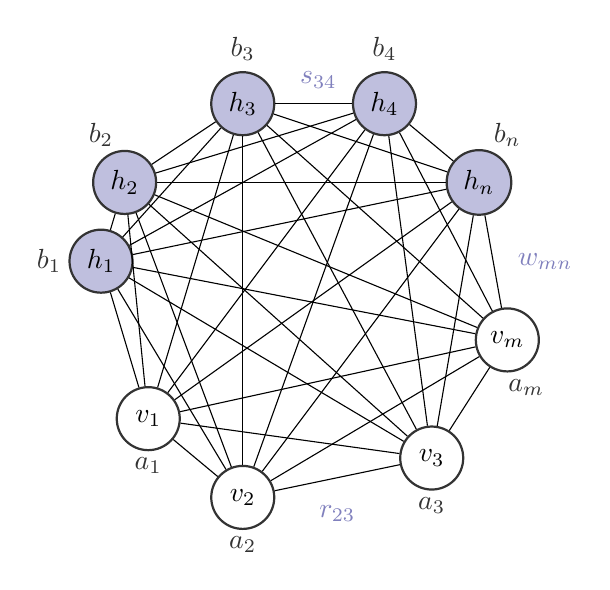
\begin{tikzpicture}
    \tikzset{cir/.style={circle,draw=black!80,thick,minimum size=0.8cm},y=0.6cm,font=\sffamily}
    \definecolor{bluebell}{rgb}{0.5, 0.5, 0.74}
    \tikzset{cirblue/.style={circle,draw=black!80,thick,
        fill=bluebell!50,minimum size=0.8cm},y=0.6cm,font=\sffamily}


    
    \begin{scope}[rotate=90]
    \node[cir] (b1) at (-2,0) {$v_1$};
    \node[cir] (b2) at (-3,-1*2) {$v_2$};
    \node[cir] (b3) at (-2.5,-3*2) {$v_3$};
    \node[cir] (b4) at (-1,-3.8*2) {$v_m$};
    \node[cirblue] (c1) at (0,1) {$h_1$};
    \node[cirblue] (c2) at (1,-1*0.5+1) {$h_2$};
    \node[cirblue] (c3) at (2,-1.5*2+1) {$h_3$};
    \node[cirblue] (c4) at (2,-3*2+1) {$h_4$};
    \node[cirblue] (c5) at (1,-3*2-1) {$h_n$};
    
    \draw (-2.6, 0) node[black!80] {$a_1$};
    \draw (-3.6, -1*2) node[black!80] {$a_2$};
    \draw (-3.1, -2*3) node[black!80] {$a_3$};
    \draw (-1.6, -4*2) node[black!80] {$a_m$};
    \draw (0, 2.1) node[black!80] {$b_1$};
    \draw (1.6, 1) node[black!80] {$b_2$};
    \draw (2.7,-1.5*2+1) node[black!80] {$b_3$};
    \draw (2.7, -3*2+1) node[black!80] {$b_4$};
    \draw (1.6,-3*2.2-1) node[black!80] {$b_n$};
    \draw (0, -4*2.1) node[bluebell!100] {$w_{mn}$};
    \draw (2.3,-2.3*2+1) node[bluebell!100] {$s_{34}$};
    \draw (-3.2,-2.5*2+1) node[bluebell!100] {$r_{23}$};
    
    
    \foreach \cnto [count=\i] in {b1,b2,b3,b4,c1,c2,c3,c4,c5} {
        \foreach \cntt [count=\j] in {b1,b2,b3,b4,c1,c2,c3,c4,c5} {
            \ifnum \i<\j
                \draw (\cnto) -- (\cntt);
            \fi
        }
    }
    
    \end{scope}
    \end{tikzpicture}
    \caption{Schematics of a BM. The nodes coloured in light purple represent the hidden layer of the network. Letters $s$ and $r$ represent the intra-layer connection, while and $w$ represents outer-layer connections.}
    \label{fig:bm}
\end{figure}






Although generative networks can be applied to various tasks, image generation serves as a practical illustration. For example, when provided with a dataset of handwritten digits, the network captures the probability distribution pattern of the pixel values. Then, after the training phase, these networks can produce samples that resemble those in the training set. 

In BMs, the training process starts by sampling the values of the hidden and visible node vectors $\mvec{h}$ and $\mvec{v}$. The inferred probability distribution is then modelled by minimising an energy function $E(\mvec{h}, \mvec{v})$ - hence the name energy-based model. More specifically, the probability is a Boltzmann distribution,
\begin{align}
    P(\mvec{h}, \mvec{v}) = \frac{\exp{(-E(\mvec{h}, \mvec{v}))} }{Z},
    \label{eq:prob_bm}
\end{align}
where $Z$ is the partition function to guarantee the probability over the whole parameter space sums to 1. This is in general an intractable function to attain. Fortunately, as discussed in \secref{sec:metropolis}, if the sampling process is done following a Metropolis algorithm, the fraction between probability distributions ensures that the partition function is in fact not necessary. More explicitly, the energy function is given by
\begin{align*}
    E(\mvec{h}, \mvec{v}) &= -\mvec{v}^\top R\mvec{v}-\mvec{v}^\top W\mvec{h}-\mvec{h}^\top S\mvec{h}-\mvec{a}^\top\mvec{v}-\mvec{b}^\top\mvec{h},
\end{align*}
where the vectors $\mvec{a}$ and $\mvec{b}$ serve as bias terms and the matrices $R$, $W$, and $S$, are modulating the connections between layers. More specifically, $R$ modulates intra-layer connections in the visible layer, $S$ plays an analogous role for the hidden layer, and $W$, between hidden and visible units. If we limit the network to only extra-layer connections, we have a restricted Boltzmann machine (RBM).

During training, the weights and biases of the model are updated aiming at maximisation of the likelihood of the model, for example via gradient descent over the negative log-likelihood.

\subsubsection{Restricted Boltzmann machines}\label{sec:rbm}

\begin{figure}[H]
    \centering
    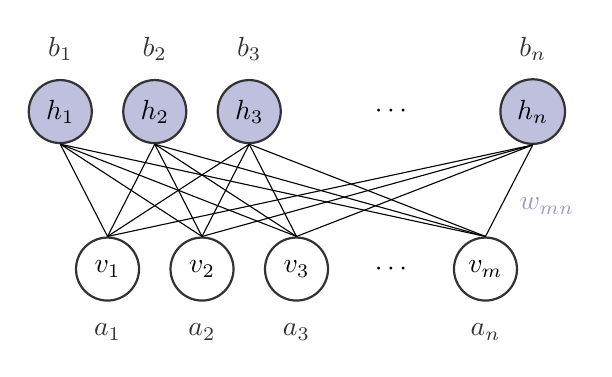
\begin{tikzpicture}
\tikzset{cir/.style={circle,draw=black!80,thick,minimum size=0.8cm},y=0.6cm,font=\sffamily}

\definecolor{bluebell}{rgb}{0.5, 0.5, 0.74}

\tikzset{cirblue/.style={circle,draw=black!80,thick,
    fill=bluebell!50,minimum size=0.8cm},y=0.6cm,font=\sffamily}

\begin{scope}[rotate=90]
\node[cir] (b1) at (0,0) {$v_1$};
\node[cir] (b2) at (0,-1*2) {$v_2$};
\node[cir] (b3) at (0,-2*2) {$v_3$};
\node[cir] (b4) at (0,-4*2) {$v_m$};
\node[cirblue] (c1) at (2,1) {$h_1$};
\node[cirblue] (c2) at (2,-1*2+1) {$h_2$};
\node[cirblue] (c3) at (2,-2*2+1) {$h_3$};
\node[cirblue] (c4) at (2,-4*2-1) {$h_n$};

\draw (-0.8, 0) node[black!80] {$a_1$};
\draw (-0.8, -1*2) node[black!80] {$a_2$};
\draw (-0.8, -2*2) node[black!80] {$a_3$};
\draw (-0.8, -4*2) node[black!80] {$a_n$};
\draw (2.8, 1) node[black!80] {$b_1$};
\draw (2.8, -1*2+1) node[black!80] {$b_2$};
\draw (2.8, -2*2+1) node[black!80] {$b_3$};
\draw (2.8, -4*2-1) node[black!80] {$b_n$};
\draw (0.8, -4*2-1.3) node[bluebell!80] {$w_{mn}$};

\foreach \i in {0,2} {
    \draw (\i,-3*2) node {$\cdots$};
}

\foreach \cnto in {1,2,3,4} {
    \foreach \cntt in {1,2,3,4} {
        \draw [-] (b\cnto.north)--(c\cntt.south);
    }
}

\end{scope}
\end{tikzpicture}
    \caption{Schematics of an RBM. Modified from the code found in \cite{stwind2020gist}.}
    \label{fig:rbm}
\end{figure}

The RBM is the generative model for which we focus part of our work. By limiting the connections of the network, we obtain what can be seen in the schematics of \figref{fig:rbm}. Regardless of this restriction, the probability function can still be expressed by  \eqref{eq:prob_bm}, while the energy term will now be, for a binary-binary ($E_{bb}$) or a Gaussian-binary case ($E_{gb}$),
\begin{align*}
    E_{bb}(\mvec{h}, \mvec{v}) &= -\mvec{v}^\top W\mvec{h}-\mvec{a}^\top\mvec{v}-\mvec{b}^\top\mvec{h}, \\
    E_{gb}(\mvec{h}, \mvec{v}) &=\frac{\norm{\mvec{v} - \mvec{a}}^2}{2\sigma^2}-\mvec{b}^\top\mvec{h} - \frac{\mvec{v}^\top W\mvec{h}}{\sigma^2}.
\end{align*}

Despite the modified architecture, the principle of training an RBM is analogous to that of BMs. However, training RBMs is considered an easier task than training other undirected models, as noted in \cite{dlbook}, because the (unnormalised) conditional $P(\mvec{h} | \mvec{v})$ can be obtained with a closed expression.

As previously touched upon, the values of the hidden and visible nodes were originally conceived as binary sampled variables, but they can also assume continuous values. This choice determines the type of the RBM, and common choices are binary-binary or Gaussian-binary. As the name implies, the former admits only binary values to both hidden and visible units, while the latter takes normally distributed variables in the visible layer.

\subsection{Feed-forward neural networks}

In its general definition, a feed-forward neural network (FFN) is a way to organise a set of compositions of parametrised functions in a sequential way.  The way nodes are organised in layers and how they are connected results in different architectures. A visual example of a common FFN setup can be seen in \figref{fig:FFN_tikz1}.

\definecolor{bluebell}{rgb}{0.5, 0.5, 0.74}
%==Begin FFN
\begin{figure}[H]
    \centering
    \begin{tikzpicture}[x=2cm,y=1cm]
      \readlist\Nnod{3,4,4,4,3} % array of number of nodes per layer
      \readlist\Nstr{n,m,m,m,k} % array of string number of nodes per layer
      \readlist\Cstr{\strut x,a^{(\prev)},a^{(\prev)},a^{(\prev)},y} % array of coefficient symbol per layer
      \def\yshift{0.5} % shift last node for dots
      
      % Define styles
      \tikzset{connect/.style={line width=0.5pt,draw=black}} % default connection style
      \tikzset{node/.style={circle, draw, minimum size=20, inner sep=0pt, outer sep=0pt, fill=white}} % default node style
      \tikzset{node grey/.style={circle, draw=black, minimum size=20, inner sep=0pt, outer sep=0pt, fill={rgb:black,2;white,10}}} % grey node style

      \message{^^J  Layer}
      \foreachitem \N \in \Nnod{ % loop over layers
        \def\lay{\Ncnt} % alias of index of current layer
        \pgfmathsetmacro\prev{int(\Ncnt-1)} % number of previous layer
        \message{\lay,}
        \foreach \i [evaluate={\c=int(\i==\N); \y=\N/2-\i-\c*\yshift;
                     \index=(\i<\N?int(\i):"\Nstr[\lay]");
                     \x=\lay; \n=\nstyle;}] in {1,...,\N}{ % loop over nodes
          % NODES
          \ifnum\lay=1
            \node[node grey] (N\lay-\i) at (\x,\y) {$\Cstr[\lay]_{\index}$};
          \else
            \ifnum\lay<\Nnodlen
              \node[node \n] (N\lay-\i) at (\x,\y) {$\Cstr[\lay]_{\index}$};
            \else
              \node[node grey] (N\lay-\i) at (\x,\y) {$\Cstr[\lay]_{\index}$};
            \fi
          \fi
          
          % CONNECTIONS
          \ifnum\lay>1 % connect to previous layer
            \foreach \j in {1,...,\Nnod[\prev]}{ % loop over nodes in previous layer
              \draw[connect] (N\prev-\j) -- (N\lay-\i);
            }
          \fi % else: nothing to connect first layer
          
        }
        \path (N\lay-\N) --++ (0,1+\yshift) node[midway,scale=1.5] {$\vdots$};
      }
      
      % LABELS
      \node[above=0.8,align=center,gray!60!black] at (N1-1.90) {input\\[-0.2em]layer};
      \node[above=0.8,align=center,bluebell!60!black] at (N3-1.90) {hidden layers};
      \node[above=0.8,align=center,gray!60!black] at (N\Nnodlen-1.90) {output\\[-0.2em]layer};
    \end{tikzpicture}
    \caption{A generic multi-layer perceptron with $n$ input nodes, $k$ output nodes and a set of three hidden layers, all with $m$ nodes. The superscript denotes the layer number, and $a$ indicates that the value has been activated by some function $\sigma$. Adapted from \cite{neutelings2021neural}}.
    \label{fig:FFN_tikz1}
\end{figure}

In contrast to an RBM, this sequence controls the flow of information, or value propagation, in one preferential direction in the network. When an FFN is said to be densely connected, each neurone receives input from all other neurones in a previous layer and, after multiplying it by a set of parameters, adding a bias value, and composing it with some activation function $\sigma$, passes the result to neurones in the next layer. This process is called a forward pass of the network and, for an L-layer deep network, is better described in \eqref{eq:FFN}:
\begin{align}
&            && \mathbf{a}^{(0)} = \mathbf{x} \notag\\
&            && 
                \negthickspace% for compensation of rcases misalignment
                \begin{rcases}  
                \mathbf{h}^{(i)}= \Vec{W}^{(i)} * \mathbf{a}^{(i-1)} + \mathbf{b}^{(i)} \notag\\
                \mathbf{a}^{(i)}    = \sigma_i(\mathbf{h}^{(i)}) 
                    \end{rcases}&  i \in \{1, ..., L-1\}, \\
&            &&\mathbf{\hat{y}} = \sigma_L(W^{(L)} *\mathbf{h}^{(L-1)} + \mathbf{b}^{(L)}).
\label{eq:FFN}
\end{align}

Here we denote $\Vec{W}^{(i)}$ and $\mathbf{b}_i$ as the weight matrix and bias vector for the i-th layer of the network.  In addition, in \eqref{eq:FFN}, $\mathbf{h}^{(i)}$ represents the output of the i-th hidden layer, while $\mathbf{a}^{(0)} = \mathbf{x}$ is the input layer. Lastly, $\sigma_i$ represents the activation function of each layer. \figref{fig:FFN_tikz2} analyses the forward pass of the first hidden layer separately to provide a better understanding of the matrix operations involved in \eqref{eq:FFN}.
\begin{figure}[H]
    \begin{tikzpicture}[x=2cm,y=1cm]
      \message{^^JNeural network activation}
      \def\NI{3} % number of nodes in input layers
      \def\NO{3} % number of nodes in output layers
      \def\yshift{0.4} % shift last node for dots
      
      % INPUT LAYE
      \foreach \i [evaluate={\c=int(\i==\NI); \y=\NI/2-\i-\c*\yshift; \index=(\i<\NI?int(\i):"n");}]
                  in {1,...,\NI}{ % loop over nodes
        \node[node in,blue!20!black!80,draw=myblue!20,fill=myblue!5, outer sep=0.6] (NI-\i) at (0,\y) {$a_{\index}^{(1)}$};
      }
      
      % OUTPUT LAYER
      \foreach \i [evaluate={\c=int(\i==\NO); \y=\NO/2-\i-\c*\yshift; \index=(\i<\NO?int(\i):"m");}]
        in {\NO,...,1}{ % loop over nodes
        \ifnum\i=1 % high-lighted node
          \node[node hidden]
            (NO-\i) at (1,\y) {$a_{\index}^{(2)}$};
          \foreach \j [evaluate={\index=(\j<\NI?int(\j):"n");}] in {1,...,\NI}{ % loop over nodes in previous layer
            \draw[connect,white,line width=1.2] (NI-\j) -- (NO-\i);
            \draw[connect] (NI-\j) -- (NO-\i)
              node[pos=0.50] {\contour{white}{$w_{1,\index}$}};
          }
        \else % other light-colored nodes
          \node[node,blue!20!black!80,draw=myblue!20,fill=myblue!5]
            (NO-\i) at (1,\y) {$a_{\index}^{(1)}$};
          \foreach \j in {1,...,\NI}{ % loop over nodes in previous layer
            %\draw[connect,white,line width=1.2] (NI-\j) -- (NO-\i);
            \draw[connect,myblue!20] (NI-\j) -- (NO-\i);
          }
        \fi
      }
      
      % DOTS
      \path (NI-\NI) --++ (0,1+\yshift) node[midway,scale=1.2] {$\vdots$};
      \path (NO-\NO) --++ (0,1+\yshift) node[midway,scale=1.2] {$\vdots$};
      
      % EQUATIONS
      \def\agr#1{{a_{#1}^{(1)}}}
      \node[below=16,right=11,mydarkblue,scale=0.95] at (NO-1)
        {$\begin{aligned} %\underset{\text{bias}}{b_1}
           &= \sigma\left(
                w_{1,1}\agr{1} + w_{1,2}\agr{2} + \ldots + w_{1,n}\agr{n} + b_1^{(1)}
              \right)\\
           &= \color{mydarkred}\sigma\left( 
                \sum_{i=1}^{n} w_{1,i}\agr{i} + b_1^{(1)}
               \right)
         \end{aligned}$};
      \node[right,scale=0.9] at (1.3,-1.3)
        {$\begin{aligned}
          {\qquad\qquad
          \begin{pmatrix}
            a_{1}^{(2)} \\[0.3em]
            a_{2}^{(2)} \\
            \vdots \\
            a_{m}^{(2)}
          \end{pmatrix}}
          &=
          \sigma\left[
          \begin{pmatrix}
            w_{1,1} & w_{1,2} & \ldots & w_{1,n} \\
            w_{2,1} & w_{2,2} & \ldots & w_{2,n} \\
            \vdots  & \vdots  & \ddots & \vdots  \\
            w_{m,1} & w_{m,2} & \ldots & w_{m,n}
          \end{pmatrix}
          {
          \begin{pmatrix}
            a_{1}^{(1)} \\[0.3em]
            a_{2}^{(1)} \\
            \vdots \\
            a_{n}^{(1)}
          \end{pmatrix}}
          +
          \begin{pmatrix}
            b_{1}^{(1)} \\[0.3em]
            b_{2}^{(1)} \\
            \vdots \\
            b_{m}^{(1)}
          \end{pmatrix}
          \right]\\[0.5em]
          &= \sigma\left( 
               \mathbf{W}^{(1)} {\mathbf{a}^{(1)}}+\mathbf{b}^{(1)}
             \right)
        \end{aligned}$};
    \end{tikzpicture}
    \caption{Forward pass between the two first layers of the network. Here, the dependency of the weight matrix elements and the connected nodes is clear, together with the activation of the affine transformation. Adapted from \cite{neutelings2021neural}.}
    \label{fig:FFN_tikz2}
\end{figure}

The activation function $\sigma$ is what allows the network, which is now our parametrised model $f_{\mvec{\theta}}(\mathbf{x})$ to express non-linear functions and learn from non-linear data, present any interesting dataset. If not for activation functions, the forward pass described in \eqref{eq:FFN} would simply be compositions of linear functions.

Common activation functions include the sigmoid function, which produces outputs between 0 and 1, the hyperbolic tangent, with outputs from -1 to 1. More recent alternatives such as the rectified linear unit (ReLU), aim at mitigating the problem of vanishing gradients. In our implementations, we opted mostly for the more recent Gaussian Error Linear Units (GELU) function \cite{hendrycks2016gaussian}, which provides enhanced performance in specific deep learning applications, and if given by
\begin{equation*}
    \text{GELU}(x) = 0.5x \left(1 + \text{erf}\left(\frac{x}{\sqrt{2}}\right)\right). 
\end{equation*}

Knowing which function to use is a complicated task and requires experimentation, as a good choice can greatly influence training efficiency and accuracy of the network.

The choice of the architecture of a network is often guided by the problem to which one aims to tackle, but most networks have some overlapping core structure in the form of the mentioned input, hidden, and output layers and activation functions. The weights and biases are then iteratively updated using a gradient scheme that tries to converge to a global minimum of the cost function $\mathcal{L}$. As mentioned in \ref{sec:Gradient-based optimisation}, this cost function is a measure of how well the model performs, be it in regression or classification problems.

\subsubsection{Training an FNN}\label{sec:training a FFN}
The task of supervised learning has some important differences from a usual minimisation problem. We are usually limited in the amount of training data, while in a minimisation problem, we might have access to the entire domain where the model should be optimised. Here we briefly describe the training of an FFN, but a more complete coverage of the topic can be found in \cite{dlbook}. Typically, we calculate and aim to minimise an average loss over a given training set, with an associated probability $\hat{p}$.
\begin{align*}
    J(\mvec{\theta}) = \mathbb{E}_{(\mvec{x}, y)\sim\hat{p}} \left[\mathcal{L}(f_{\mvec{\theta}}(\mvec{x}), y)\right],
\end{align*}

Within the empirical risk minimisation framework, we hope that by minimising this expected value, we will effectively generalise the probability distribution of the true data $p$. We intentionally do not focus much on this aspect, as in VMC there is no explicit separation between training and test sets. As this expectation value is empirically just an average in the training set, we sometimes use $\nabla \mathcal{L}$ and $\nabla J$ interchangeably.

Regardless of the loss of the model, the training process of an FFN will involve the following steps. First, we perform a forward pass to generate predictions. Next, we evaluate these predictions and compute the gradient of the loss function with respect to the parameters. Then, with this gradient information, we update the parameters accordingly, with any of the methods described in the section on gradient-based optimisation \secref{sec:Gradient-based optimisation}.

To ensure that the loss information flows backward through the network and updates the parameters correctly, we must consider the function compositions in \eqref{eq:FFN} due to different layers in the network. This involves correct application of the chain rule during the gradient evaluations of $\nabla_{\mvec{\theta}} \mathcal{L}$, which will in fact depend on the activation functions that are used.

To handle flexible and arbitrary networks, gradients are often computed using automatic differentiation, which we explain in more detail in \secref{sec:ad}. This approach can sometimes obscure the backward propagation step. For clarity, we provide a simplified mathematical overview of the backpropagation equations, the demonstrations of which are available in Nielsen (2015) \cite{nielsen2015neural}. The gradient of the loss function with respect to the weights and biases of layer $i$ are given by 
\begin{align}
    \nabla_{\Vec{W}^{(i)}} \mathcal{L} &= \delta^{(i)} (\mathbf{a}^{(i-1)})^\top \label{eq:nabla_weight}\\
    \nabla_{\mathbf{b}^{(i)}} \mathcal{L} &= \delta^{(i)},\label{eq:nabla_bias}
\end{align}
where $\delta^{(i)}$ represents a measure of the loss at layer $i$, given by 
\begin{equation*}
  \delta^{(i)} = \begin{cases}
    \nabla_{\mathbf{\hat{y}}} \mathcal{L} \odot \sigma'_L(\mathbf{h}^{(L)}) & \text{if } i = L, \\
    (\Vec{W}^{(i+1)})^\top \delta^{(i+1)} \odot \sigma'_i(\mathbf{h}^{(i)}) & \text{if } i < L.
  \end{cases}
\end{equation*}

Due to the chain rule evaluation order, $\delta^{(i)}$ depends on $\delta^{(i+1)}$ and we must start from the last layer and progress inward. The expressions further simplify given the knowledge of the activation functions $\sigma$. A depiction of the training is given by Algorithm \ref{algo:ffn_train}.

\begin{algorithm}[H]
    \caption{Training a Feedforward Neural Network}
    \begin{algorithmic} 
    \STATE \textbf{Input:} Training data $(\mathbf{x}, \mathbf{y})$, initialized weights $\mathbf{W}^{(i)}$, biases $\mathbf{b}^{(i)}$, and learning rate $\alpha$
    \FOR{each training iteration}
        \STATE \textbf{Forward Pass:}
        \FOR{each layer $i \in \{1, \ldots, L-1\}$}
            \STATE Compute pre-activation: $\mathbf{h}^{(i)} = \mathbf{W}^{(i)} \mathbf{a}^{(i-1)} + \mathbf{b}^{(i)}$
            \STATE Compute activation: $\mathbf{a}^{(i)} = \sigma_i(\mathbf{h}^{(i)})$
        \ENDFOR
        \STATE Compute output: $\mathbf{\hat{y}} = \sigma_L(\mathbf{W}^{(L)} \mathbf{h}^{(L-1)} + \mathbf{b}^{(L)})$
        \STATE Computate loss: $\mathcal{L}(\mathbf{\hat{y}}, \mathbf{y})$
        \STATE \textbf{Backward Pass:}
        \STATE Compute output layer error: $\delta^{(L)}$
        \FOR{each layer $i \in \{L-1, \ldots, 1\}$}
            \STATE Backpropagate error: $\delta^{(i)}$
        \ENDFOR
        \STATE \textbf{Gradient Computation:}
        \FOR{each layer $i \in \{1, \ldots, L\}$}
            \STATE Compute gradients $\nabla_{\mathbf{W}^{(i)}} \mathcal{L}$ and $\nabla_{\mathbf{b}^{(i)}} \mathcal{L}$
        \ENDFOR
        \STATE \textbf{Parameter Update:}
        \FOR{each layer $i \in \{1, \ldots, L\}$}
            \STATE Update weights: $\mathbf{W}^{(i)} \leftarrow \mathbf{W}^{(i)} - \alpha \nabla_{\mathbf{W}^{(i)}} \mathcal{L}$
            \STATE Update biases: $\mathbf{b}^{(i)} \leftarrow \mathbf{b}^{(i)} - \alpha \nabla_{\mathbf{b}^{(i)}} \mathcal{L}$
        \ENDFOR
        \STATE Check for convergence or stopping criteria
    \ENDFOR
\end{algorithmic}
\label{algo:ffn_train}
\end{algorithm}


\subsubsection{A comment on the capabilities of ANNs}

When talking about the learning capabilities of neural networks, we must mention universal approximation theorems. ANNs are compositions of parametrised functions, but how can one ensure that they are capable of approximating an ideal model $\hat{f}$, directing the statistics of the observed data? In fact, there are a set of universality theorems which provide this guarantee under certain conditions.

Cybenko showed in 1989 \cite{cybenko1989approximation} that multi-layer perceptrons with sigmoid functions can approximate any continuous function. The theorem, proven for at least one hidden layer, does not mention any constraint on the number of epochs or neurones required. This means that such universality could in practice be infeasible. Further developed theorems exist that eliminate the requirement of a sigmoid activation function \cite{can1991multilayer}, and others have shown that the universal approximation theorem also applies to convolutional networks, recurrent networks, and more recently graph neural networks \cite{zhou2020universality, schafer2006recurrent, bruel2020universal}.

Being able to approximate an arbitrary function is only half the problem. Why would such a model be able to generalise to unseen data? To quote R. Grosse (2021) \cite{grosse2021csc2541}: ``After all, the optimisation landscape is non-convex, highly non-linear, and high-dimensional, so why are we able to train these networks? In many cases, they have far more than enough parameters to memorize the data, so why do they generalise well? [...] the attitude of the neural net community was to train first and ask questions later. Apparently, this worked.''

In practice, even if the convergence of a problem is not guaranteed, we often reach ``good enough'' solutions with NNs. It is not uncommon to use methods for which there is no theoretically solid argument other than documented success. Fortunately, theoretical proofs have so far been presented in the years that follow.

\section{Reinforcement Learning and VMC}\label{sec:VMC_RL}

Various forms of reinforcement learning (RL) exist, yet they all address an optimisation problem with the concept of agents. These agents, through a set of actions $\mathcal{A} = \{a_t\}$, are able to influence the environment states $\mathcal{S} = \{s_t\}$. Their goal is to maximise the accumulation of immediate rewards $r_{a_{t}}(s_t, s')$ for adopting a state $s'$.

Contrary to supervised learning, in which the stream of input for a model comes from a fixed data set, in reinforcement learning, such a dataset is iteratively dependent on the previous samples. In this sense, we say that the agent interacts and changes the environment, making more explicit the need for balance between exploration and exploitation to train a model.

To try and maximise a cumulative reward, an agent can take random actions to explore configuration space (exploration), but also use information from current and previous decisions to be rewarded (exploitation). Too much exploration leads to multiple sub-optimal choices, while too much exploitation results in local minima from limited prior knowledge.

In VMC, there is an element of exploration when modelling a probability distribution by accepting steps with a guided acceptance rule. Furthermore, VMC uses information from previous samples to minimise the expected value of the local energy, which is cumulative by construction. Not occasionally, reinforcement learning can be modelled by a Markov process, with an associated transition probability $t_a(s, s')$ from $s$ to $s'$ under an action $a$.

The goal of RL agents is to learn a parametrised policy distribution $\pi_{\mvec{\theta}}: \mathcal{A} \times \mathcal{S} \to [0,1]$, which, once optimised, will produce a stationary Markov chain distribution that maximises the expected cumulative reward over time. Consider the Markov chain of state and action $\tau_t = (s_t, a_t)$. There are several ways of measuring this expected cumulative reward, one of which being
\begin{align*}
    \mathcal{J}(\mvec{\theta})&= \mathbb{E}_{\tau \sim \pi_{\mvec{\theta}}} \left[G_t\right] \\
    G_t &= \sum_{k=0}^\infty \gamma^k r_{a_{t+ k + 1}}
\end{align*}
with $\gamma \in [0, 1)$ a discount return rate, so that immediate rewards are more important for step $t$ than ones far in the future. This expectation value is usually computed via Monte Carlo averaging, and there are multiple approaches to optimise this reward, such as gradient ascent, with neural networks as agents. Then, it can be shown \cite{sutton2018reinforcement} that
\begin{align*}
    \nabla_{\mvec{\theta}} \mathcal{J}({\mvec{\theta}})&\propto \mathbb{E}_{\pi_{\mvec{\theta}}} \left[G_t\nabla_{\mvec{\theta}}\ln\pi_{\mvec{\theta}}(\tau)\right].
\end{align*}

Unfortunately, and this is a problem we also face in VMC, the gradients of expectation values of the estimated loss/reward function have very high variance, motivating the use of approximate second-order methods like NGD, but also techniques like the REINFORCE \cite{williams1992simple} and a variance reduction technique called the baseline method. When these are used, the gradient is calculated in a more stable way \cite{dlbook} by subtracting a baseline $b({\mvec{\theta}})$
\begin{align*}
    \nabla_{\mvec{\theta}} \mathcal{J}(\mvec{\theta})&\propto \mathbb{E}_{\tau \sim \pi_{\mvec{\theta}}} \left[(G_t - b(\mvec{\theta}))\nabla_{\mvec{\theta}} \ln \pi_{\mvec{\theta}}(\tau) \right],
\end{align*}
where $b$ is simply an offset that does not depend on on the action. There are techniques to further find the baseline to best reduce the variance, but it is sometimes simply set as the expected reward $\mathcal{J}(\mvec{\theta})$. Here we see a stark parallel between the gradient of the cumulative reward and the gradient of the expected local energy of the quantum system:
\begin{equation*}
    \nabla_{\mvec{\theta}} E(\mvec{\theta})=2 \mathbb{E}_{\mathbf{R}\sim |\psi_\theta|^2}\left[ \left(E_L
- E(\mvec{\theta})\right)\nabla_{\mvec{\theta}}\ln \Psi_{\mvec{\theta}} (\mathbf{R})\right].
\label{eq:grad_el_vmc}
\end{equation*}

At this point, we see it is at least possible to adapt RL methods to improve the VMC scheme. Evidently, some dissimilarities must also be mentioned. As noted in \cite{sheng}, the gradient expressions in VMC involve quantum amplitudes instead of probability, and furthermore, the probability of the quantum state is often not normalised. However, the analogy between neural network reinforcement learning and VMC remains. Here, the neural networks that suggest quantum states act as agents, with the environments offering feedback in the form of the energy of the state. The parameters are then adjusted to minimise this energy, implying that the reward can correspond to the negative of the local energy.

\subsection{Neural Quantum States}\label{sec:NQS}

In 2017, Carleo and Troyer were the first to introduce a method in which larger neural networks are used as a variational ansatz for quantum states \cite{carleo2017solving}. The method, which they called neural quantum states (NQS), was conceptualised using a restricted Boltzmann machine as the network, aiming at solving interacting spins models. Now, NQSs have been applied to a large set of physical problems and using many common types of neural networks, such as feed-forward, convolutional, recurrent, graph neural networks, and more \cite{lange2024architectures}. At the core of these methods is a variational minimisation task under a reinforcement learning framework.

Similar variational ansätze, such as matrix product states \cite{orus2014practical}, have been used previously, but with limited generalisability to different quantum systems. The motivation for employing neural networks is rooted in their representational power, as guaranteed by universal approximation theorems, combined with their capacity for dimensionality reduction. In fact, the field of machine learning has faced challenges analogous to those of quantum mechanics when it comes to the curse of dimensionality.

To describe neural quantum states, we follow \cite{lange2024architectures} and proceed in a similar way to our VMC section, \secref{sec:VMC}. A general state in a basis set of the possible configurations $\{\ket{\mvec{\sigma}}\}$ is written
\begin{equation*}
\ket{\psi} = \sum_{\mvec{\sigma}}\psi(\mvec{\sigma}) \ket{\mvec{\sigma}},
\end{equation*}
where $\mvec{\sigma}$ could be spin configurations, as posed originally by Carleo, or positions, in our case. Then, different configurations are sampled and are the inputs to the network, which serve as the coefficients $\psi(\mvec{\sigma})$. The neural quantum states can be expressed as 
\begin{equation*}
    \psi_{\theta}(\mvec{\sigma}) = \sqrt{p_{\mvec{\theta}}(\mvec{\sigma})} e^{i\phi_{\mvec{\theta}}(\mvec{\sigma})},
\end{equation*}
with amplitude $p_{\mvec{\theta}}(\mvec{\sigma}) = |\psi_{\mvec{\theta}}(\mvec{\sigma})|^2$ and phase $\phi_{\mvec{\theta}}(\mvec{\sigma}) = \text{Im}(\ln \psi_{\mvec{\theta}} (\mvec{\sigma}))$. Different methods exist for handling the phase of the wavefunction. One approach involves using two distinct networks or separate outputs: one for the imaginary component and another for the real component. Alternatively, the network can be trained with complex parameters. This approach increases the size of the parameter space, and since we deal with bounded and time-independent systems, we chose to disregard the imaginary part of the wavefunction altogether.

Then, the expectation values of observables are approximated via Monte Carlo averaging, in complete analogy to the variational Monte Carlo approach:
\begin{equation*}
    \langle\hat{O}\rangle \approx  \sum_{\mvec{\sigma}} P_{\mvec{\theta}}(\mvec{\sigma}) O_{L,\mvec{\theta}}(\mvec{\sigma}),
\end{equation*}
with the normalized configuration probability $P_{\mvec{\theta}}(\mvec{\sigma})$ and the local operator estimator, $O_{L,\mvec{\theta}}(\mvec{\sigma})$ already defined in \secref{sec:VMC}. Again, if one uses sampling algorithms such as Metropolis, the ansätze used in the sampling need not be normalised - which is very useful for deep networks, where calculating the partition function is difficult.

Training an NQS, as most of the interesting machine learning problems, is a non-convex task. Therefore, machine learning techniques and optimisers are beneficial in the parameter update routine. A generic NQS training algorithm is shown in Algorithm \ref{algo:nqs_update_rule}, where we show that NQSs are trained without the use of external training data. In the displayed case, we use the space configurations of the system, $\mvec{\sigma} = \mathbf{R}$.

The details of our specific RBM, FFN and Deep Set FFN implementations, together with the standard VMC ansatz, can be seen in the Methods part, \secref{sec:ansatz_closer_view}.

\begin{algorithm}[H]
    \caption{Neural Network VMC with MCMC Sampling. The parameters $\mvec{\theta}$ are updated based on the local energy $E_L(\Vec{R}_i)$ calculated for sampled configurations. The Metropolis acceptance ratio $A$ and uniform probability distributions $U_c$ are used to accept or reject proposed configurations. All particles are moved at once.}
    \label{algo:nqs_update_rule}
    \begin{algorithmic}
        \STATE Initialize the state parameters and position $\psi_{\mvec{\theta}}(\mathbf{R}) \leftarrow \mvec{\theta}_0, \, \mathbf{R}_0$ 
        \FOR{each epoch}
            \FOR{each MCMC step}
                \STATE $\Vec{R}' \leftarrow$ Propose new configuration based on $\Vec{R}$ and $\mvec{\theta}$
                \STATE $A \leftarrow$ Compute Metropolis acceptance ratio $A(\Vec{R} \rightarrow \Vec{R}') = \min\left(1, \frac{|\Psi_{\mvec{\theta}} (\Vec{R}')|^2}{|\Psi_{\mvec{\theta}}(\Vec{R})|^2}\right).$
                \STATE $r \sim U_c(0,1)$ (Draw uniform number)
                \IF{$A \geq r \text{ (Acceptance criteria)}$} 
                    \STATE $\Vec{R} \leftarrow \Vec{R}'$ (Accept new configuration)
                \ENDIF
            \ENDFOR
            \STATE $\{\Vec{R}_i\} \leftarrow$ Sample batch of configurations by MCMC
            \STATE $E_L(\Vec{R}_i) \leftarrow$ Calculate local energy for each $\Vec{R}_i$
            \STATE $\nabla_{\mvec{\theta}} \langle E_L\rangle \leftarrow$ Compute gradient with respect to $\mvec{\theta}$
            \STATE $\mvec{\theta} \leftarrow \mvec{\theta} - \alpha \nabla_{\mvec{\theta}} \langle E_L\rangle$ Update parameters
            \STATE Check for convergence or stopping criteria
        \ENDFOR
    \end{algorithmic}
\end{algorithm}
